\documentclass{article}

  % packages
    % basic stuff for rendering math
    \usepackage[letterpaper, top=1in, bottom=1in, left=1in, right=1in]{geometry}
    \usepackage[utf8]{inputenc}
    \usepackage[english]{babel}
    \usepackage{amsmath} 
    \usepackage{amssymb}
    % \usepackage{amsthm}

    % extra math symbols and utilities
    \usepackage{mathtools}        % for extra stuff like \coloneqq
    \usepackage{mathrsfs}         % for extra stuff like \mathsrc{}
    \usepackage{centernot}        % for the centernot arrow 
    \usepackage{bm}               % for better boldsymbol/mathbf 
    \usepackage{bbm}               % for better boldsymbol/mathbf 
    \usepackage{enumitem}         % better control over enumerate, itemize
    \usepackage{hyperref}         % for hypertext linking
    \usepackage{fancyvrb}          % for better verbatim environments
    \usepackage{newverbs}         % for texttt{}
    \usepackage{xcolor}           % for colored text 
    \usepackage{listings}         % to include code
    \usepackage{lstautogobble}    % helper package for code
    \usepackage{parcolumns}       % for side by side columns for two column code
    

    % page layout
    \usepackage{fancyhdr}         % for headers and footers 
    \usepackage{lastpage}         % to include last page number in footer 
    \usepackage{parskip}          % for no indentation and space between paragraphs    
    \usepackage[T1]{fontenc}      % to include \textbackslash
    \usepackage{footnote}
    \usepackage{etoolbox}

    % for custom environments
    \usepackage{tcolorbox}        % for better colored boxes in custom environments
    \tcbuselibrary{breakable}     % to allow tcolorboxes to break across pages

    % figures
    \usepackage{pgfplots}
    \pgfplotsset{compat=1.18}
    \usepackage{float}            % for [H] figure placement
    \usepackage{tikz}
    \usepackage{tikz-cd}
    \usepackage{circuitikz}
    \usetikzlibrary{arrows}
    \usetikzlibrary{positioning}
    \usetikzlibrary{calc}
    \usepackage{graphicx}
    \usepackage{caption} 
    \usepackage{subcaption}
    \captionsetup{font=small}

    % for tabular stuff 
    \usepackage{dcolumn}

    \usepackage[nottoc]{tocbibind}
    \pdfsuppresswarningpagegroup=1
    \hfuzz=5.002pt                % ignore overfull hbox badness warnings below this limit

  % New and replaced operators
    \DeclareMathOperator{\Tr}{Tr}
    \DeclareMathOperator{\Sym}{Sym}
    \DeclareMathOperator{\ARMA}{ARMA}
    \DeclareMathOperator{\Span}{span}
    \DeclareMathOperator{\std}{std}
    \DeclareMathOperator{\Cov}{Cov}
    \DeclareMathOperator{\Var}{Var}
    \DeclareMathOperator{\Corr}{Corr}
    \DeclareMathOperator{\pos}{pos}
    \DeclareMathOperator*{\argmin}{\arg\!\min}
    \DeclareMathOperator*{\argmax}{\arg\!\max}
    \newcommand{\ket}[1]{\ensuremath{\left|#1\right\rangle}}
    \newcommand{\bra}[1]{\ensuremath{\left\langle#1\right|}}
    \newcommand{\braket}[2]{\langle #1 | #2 \rangle}
    \newcommand{\qed}{\hfill$\blacksquare$}     % I like QED squares to be black

  % Custom Environments
    \newtcolorbox[auto counter, number within=section]{question}[1][]
    {
      colframe = orange!25,
      colback  = orange!10,
      coltitle = orange!20!black,  
      breakable, 
      title = \textbf{Question \thetcbcounter ~(#1)}
    }

    \newtcolorbox[auto counter, number within=section]{exercise}[1][]
    {
      colframe = teal!25,
      colback  = teal!10,
      coltitle = teal!20!black,  
      breakable, 
      title = \textbf{Exercise \thetcbcounter ~(#1)}
    }
    \newtcolorbox[auto counter, number within=section]{solution}[1][]
    {
      colframe = violet!25,
      colback  = violet!10,
      coltitle = violet!20!black,  
      breakable, 
      title = \textbf{Solution \thetcbcounter}
    }
    \newtcolorbox[auto counter, number within=section]{lemma}[1][]
    {
      colframe = red!25,
      colback  = red!10,
      coltitle = red!20!black,  
      breakable, 
      title = \textbf{Lemma \thetcbcounter ~(#1)}
    }
    \newtcolorbox[auto counter, number within=section]{theorem}[1][]
    {
      colframe = red!25,
      colback  = red!10,
      coltitle = red!20!black,  
      breakable, 
      title = \textbf{Theorem \thetcbcounter ~(#1)}
    } 
    \newtcolorbox[auto counter, number within=section]{proposition}[1][]
    {
      colframe = red!25,
      colback  = red!10,
      coltitle = red!20!black,  
      breakable, 
      title = \textbf{Proposition \thetcbcounter ~(#1)}
    } 
    \newtcolorbox[auto counter, number within=section]{corollary}[1][]
    {
      colframe = red!25,
      colback  = red!10,
      coltitle = red!20!black,  
      breakable, 
      title = \textbf{Corollary \thetcbcounter ~(#1)}
    } 
    \newtcolorbox[auto counter, number within=section]{proof}[1][]
    {
      colframe = orange!25,
      colback  = orange!10,
      coltitle = orange!20!black,  
      breakable, 
      title = \textbf{Proof. }
    } 
    \newtcolorbox[auto counter, number within=section]{definition}[1][]
    {
      colframe = yellow!25,
      colback  = yellow!10,
      coltitle = yellow!20!black,  
      breakable, 
      title = \textbf{Definition \thetcbcounter ~(#1)}
    } 
    \newtcolorbox[auto counter, number within=section]{example}[1][]
    {
      colframe = blue!25,
      colback  = blue!10,
      coltitle = blue!20!black,  
      breakable, 
      title = \textbf{Example \thetcbcounter ~(#1)}
    } 
    \newtcolorbox[auto counter, number within=section]{code}[1][]
    {
      colframe = green!25,
      colback  = green!10,
      coltitle = green!20!black,  
      breakable, 
      title = \textbf{Code \thetcbcounter ~(#1)}
    } 

    \BeforeBeginEnvironment{example}{\savenotes}
    \AfterEndEnvironment{example}{\spewnotes}
    \BeforeBeginEnvironment{lemma}{\savenotes}
    \AfterEndEnvironment{lemma}{\spewnotes}
    \BeforeBeginEnvironment{theorem}{\savenotes}
    \AfterEndEnvironment{theorem}{\spewnotes}
    \BeforeBeginEnvironment{corollary}{\savenotes}
    \AfterEndEnvironment{corollary}{\spewnotes}
    \BeforeBeginEnvironment{proposition}{\savenotes}
    \AfterEndEnvironment{proposition}{\spewnotes}
    \BeforeBeginEnvironment{definition}{\savenotes}
    \AfterEndEnvironment{definition}{\spewnotes}
    \BeforeBeginEnvironment{exercise}{\savenotes}
    \AfterEndEnvironment{exercise}{\spewnotes}
    \BeforeBeginEnvironment{proof}{\savenotes}
    \AfterEndEnvironment{proof}{\spewnotes}
    \BeforeBeginEnvironment{solution}{\savenotes}
    \AfterEndEnvironment{solution}{\spewnotes}
    \BeforeBeginEnvironment{question}{\savenotes}
    \AfterEndEnvironment{question}{\spewnotes}
    \BeforeBeginEnvironment{code}{\savenotes}
    \AfterEndEnvironment{code}{\spewnotes}

    \definecolor{dkgreen}{rgb}{0,0.6,0}
    \definecolor{gray}{rgb}{0.5,0.5,0.5}
    \definecolor{mauve}{rgb}{0.58,0,0.82}
    \definecolor{lightgray}{gray}{0.93}

    % default options for listings (for code)
    \lstset{
      autogobble,
      frame=ltbr,
      language=C,                           % the language of the code
      aboveskip=3mm,
      belowskip=3mm,
      showstringspaces=false,
      columns=fullflexible,
      keepspaces=true,
      basicstyle={\small\ttfamily},
      numbers=left,
      firstnumber=1,                        % start line number at 1
      numberstyle=\tiny\color{gray},
      keywordstyle=\color{blue},
      commentstyle=\color{dkgreen},
      stringstyle=\color{mauve},
      backgroundcolor=\color{lightgray}, 
      breaklines=true,                      % break lines
      breakatwhitespace=true,
      tabsize=3, 
      xleftmargin=2em, 
      framexleftmargin=1.5em, 
      stepnumber=1
    }

  % Page style
    \pagestyle{fancy}
    \fancyhead[L]{Frequentist Statistics}
    \fancyhead[C]{Muchang Bahng}
    \fancyhead[R]{December 2022} 
    \fancyfoot[C]{\thepage / \pageref{LastPage}}
    \renewcommand{\footrulewidth}{0.4pt}          % the footer line should be 0.4pt wide
    \renewcommand{\thispagestyle}[1]{}  % needed to include headers in title page

\begin{document}

\title{Frequentist Inference}
\author{Muchang Bahng}
\date{Winter 2022}

\maketitle
\tableofcontents
\pagebreak

This covers computability theory, complexity theory, and automata theory. 
Alphabet. Boolean logic


\section{Point Estimation}

  \begin{definition}[Sample Statistic, Estimators and Estimates]
    Now given a population $X$, we would like to use the $n$ iid samples $x_1, \ldots, x_n$ to estimate a parameter $\theta$ of interest with our own random variable/value $\widehat{\theta}_n$, called a \textbf{sample statistic}. We must note the dual nature of the sample statistic as a random variable and a value is similar to that of samples. 
    \begin{enumerate}
      \item The statistic $\widehat{\theta}_n$ is a random variable itself, referred to as the \textbf{estimator}. More specifically, it is a function $\widehat{\theta}_n: \mathbb{R}^n \longrightarrow \mathbb{R}$ of the $n$ samples, i.e. a transformation of random variables 
      \begin{equation}
        \widehat{\theta}_n = \widehat{\theta}_n (x_1, x_2, \ldots, x_n)
      \end{equation}
      This makes $\widehat{\theta}_n$ also a random variable, which attempts to estimate the true $\theta$, which is some unknown fixed value. Since $\widehat{\theta}_n$ is a random variable, it has its own distribution, called the \textbf{sampling distribution} of $\widehat{\theta}_n$. 
      
      \item Once these samples $x_i$ have been realized, the estimator realizes and the value realized is now called the \textbf{estimate}. 
    \end{enumerate}
    This sampling distribution is a distribution of the statistic $\widehat{\theta}_n$, and this forms a separate distribution with its own mean and variance. 
    \begin{enumerate}
      \item the mean of the sampling distribution is denoted $\mu_{\widehat{\theta}_n}$
      \item the standard deviation of the sampling distribution is denoted $\sigma^2_{\widehat{\theta}_n}$, also called the \textbf{standard error}. 
    \end{enumerate}
  \end{definition}

  We would want these estimators to have three properties: 
  \begin{enumerate}
    \item unbiasedness
    \item consistency 
    \item efficiency
  \end{enumerate}

  We would like the sampling distribution of our statistic to give us good estimate in two ways. $\widehat{\theta}_n$ should not be too far off from the actual parameter $\theta$ (bias is small), and $\widehat{\theta}_n$ should not fluctuate too widely (variance of $\widehat{\theta}_n$ should be small). 

  \begin{definition}[Bias, Variance of Estimator]
    Given an estimator $\widehat{\theta}$ of a sample $x_1, \ldots, x_n$ estimating population parameter $\theta$, the \textbf{sampling bias} refers to 
    \begin{equation}
      \mathrm{Bias}(\widehat{\theta}) = \big| \mathbb{E}[\widehat{\theta}] - \theta \big|
    \end{equation}
    and the \textbf{sampling variance} refers to 
    \begin{equation}
      \mathrm{Var}(\widehat{\theta}) = \mathbb{E} \big[ (\widehat{\theta} - \mathbb{E}[\widehat{\theta}])^2 \big]
    \end{equation}
  \end{definition}

  A good rule of thumb to remember is that statistics is about replacing expectations with averages. 
  \begin{equation}
    \mathbb{E} \mapsto \frac{1}{n} \sum_i
  \end{equation}
  This is really the fundamental quality of statistics. Then after that we can do some fancy things, like minimizing something or manipulating another, but every single time we see an expectation just replace it with an average. 

  \begin{definition}[Sample Mean]
    Given a population $X$ with $\mu = \mathbb{E}[X]$ and $\sigma^2 = \mathrm{Var}(X)$, our estimator for $\mu$ is simply the average of the $n$ samples $x_1, \ldots, x_n$, called the \textbf{sample mean} or the \textbf{sampling distribution of the sample mean}. 
    \begin{equation}
      \overline{x}_n = \widehat{\mu}_n = \frac{1}{n} (x_1 + \ldots + x_n)
    \end{equation}
    This gives us the sampling distribution of the sample means. The mean and standard deviation (i.e. standard error) of $\overline{x}_n$ is denoted $\mu_{\overline{x}_n}$ and $\sigma_{\overline{x}_n}$. 
    \begin{enumerate}
      \item The mean of $\overline{x}_n$ is $\mu$. 
      \begin{equation}
        \mu_{\overline{x}_n} = \mu
      \end{equation}
      because
      \begin{equation}
        \mathbb{E}[\overline{x}_n] = \mathbb{E} \bigg[ \frac{1}{n} \sum_{i=1}^n x_i \bigg] = \frac{1}{n} \sum_{i=1}^n \mathbb{E}[x_i] = \mathbb{E}[x] = \mu
      \end{equation}
      
      \item The variance of $\overline{x}_n$ is $\sigma^2 / n$, i.e. the standard error of $\overline{x}_n$ is $\sigma_{\overline{x}_n} = \sigma / \sqrt{n}$. 
      \begin{equation}
        \sigma_{\overline{x}_n} = \frac{\sigma}{\sqrt{n}}
      \end{equation}
      because 
      \begin{equation}
        \sigma^2_{\overline{x}_n} = \frac{1}{n^2} \sum_{i=1}^n \mathrm{Var}(x_i) = \frac{1}{n} \mathrm{Var}(x) = \frac{\sigma^2}{n}
      \end{equation}
       Practically, this tells us that when trying to estimate the value of a population mean, due to the factor of $1/\sqrt{n}$, reducing the error on the estimate by a factor of $2$ requires acquiring $4$ times as many observations in the sample. But realistically, the true standard deviation $\sigma$ is unknown, and so the standard error of the mean is usually estimated by replacing $\sigma$ with the sample standard deviation $S$ instead. 
      \begin{equation}
        \sigma_{\overline{x}_n} \approx \frac{S}{\sqrt{n}}
      \end{equation}

      \item By CLT, $\overline{x}_n$ converges to $\mathcal{N}(\mu, \sigma^2/n)$ in distribution as $n \rightarrow +\infty$ (but in practicality, we assume this for $n \geq 30$). The fact that its mean and variance is $\mu$ and $\sigma^2 /n$ isn't that impressive. What is really impressive is that no matter what the distribution of $x$ is, the sampling distribution of the mean will be Gaussian. 
    \end{enumerate}
  \end{definition}

  \begin{example}[Sample Means]
    Here are some figures of sample means. Note that with a uniform parent distribution, the sampling distribution of its mean looks like a Gaussian even without a large $n$. However, this is not necessarily true for different parent distributions, such as the exponential. 
    \begin{figure}[H]
      \centering
      \begin{subfigure}[b]{0.48\textwidth}
      \centering
        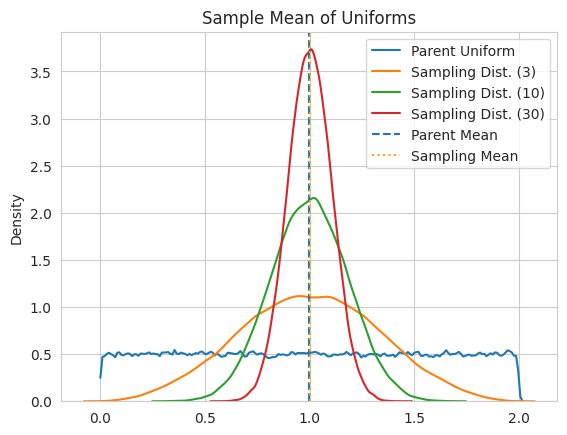
\includegraphics[width=\textwidth]{img/sample_mean_uniform.png}
        \caption{We plot the PDF of an $X \sim \mathrm{Uniform}[0, 2]$ random variable by taking 100k samples. We also take 100k samples from the sampling distribution of the mean $\overline{X}_{3}, \overline{X}_{10}, \overline{X}_{30}$. We can see that the standard deviation decreases by a factor of $\sqrt{n}$.}
        \label{fig:sample_mean_uniform}
      \end{subfigure}
      \hfill 
      \begin{subfigure}[b]{0.48\textwidth}
      \centering
        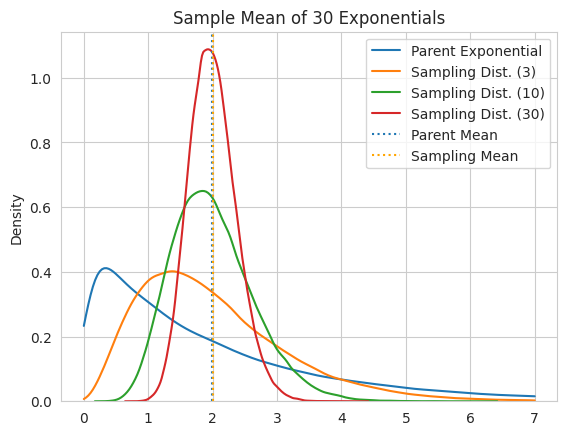
\includegraphics[width=\textwidth]{img/sample_mean_exp.png}
        \caption{We plot the PDF of an $X \sim \mathrm{Exponential}(1.5)$ random variable by taking 100k samples. We also take 100k samples from the sampling distribution of the mean $\overline{X}_{3}, \overline{X}_{10}, \overline{X}_{30}$. }
        \label{fig:sample_mean_exp}
      \end{subfigure}
      \caption{}
      \label{fig:sample_mean_examples}
    \end{figure}
  \end{example}

  If the parent distribution is normal, then we don't even need CLT to claim that the sampling distribution of the sample mean is normal, since sums of normals are normal. 

  Now the variance of the population is defined to be $\sigma^2 = \mathbb{E}[ (X - \mathbb{E}[X])^2 ]$, and by our rule of thumb, we can replace the expectations with sample means, by first setting $\mathbb{E}[X] = \widehat{\mu}$ and averaging out the values $(X - \widehat{\mu})^2$. 

  \begin{definition}[Sample Variance]
    Given a population $X$, our estimator for $\sigma^2 = \mathbb{E}[ (X - \mathbb{E}[X])^2 ]$ is simply the average of the squared distances of the $n$ samples $\{(x_i - \widehat{\mu})^2\}_{i=1}^n$. 
    \begin{equation}
      S^2_n = \widehat{\sigma}^2_n = \frac{1}{n} \sum_{i=1}^n ( x_i - \overline{x}_n)^2
    \end{equation}
    The mean and standard deviation of $S^2_n$ is denoted $\mu_{S^2_n}$ and $\sigma_{S^2_n}$. Note that there is a small difference that the sum for variance is divided by $n-1$ rather than $n$, since we want it to be unbiased, but we will correct this later. 
  \end{definition}

  While the CLT states that the sampling distribution of the sample mean will look approximately Gaussian, we do not have this luxury when looking at the sampling distribution of sample variance. 

  \begin{example}[Sample Variance]
    Take a look at the following sampling distributions of the sample variance. There does not seem to be strong signs of convergence to a Gaussian. Their means do not align either. 
    \begin{figure}[H]
      \centering
      \begin{subfigure}[b]{0.48\textwidth}
      \centering
        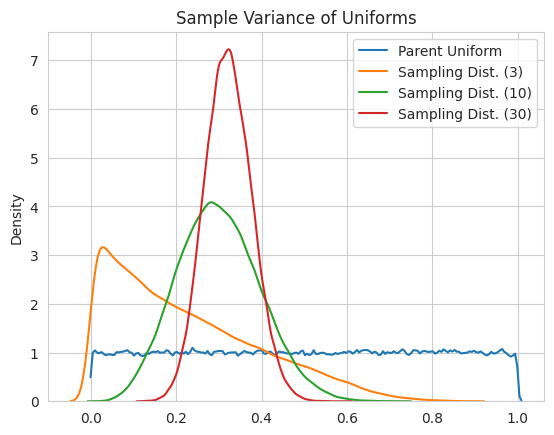
\includegraphics[width=\textwidth]{img/sample_variance_uniform.png}
        \caption{}
        \label{fig:sample_variance_uniform}
      \end{subfigure}
      \hfill 
      \begin{subfigure}[b]{0.48\textwidth}
      \centering
        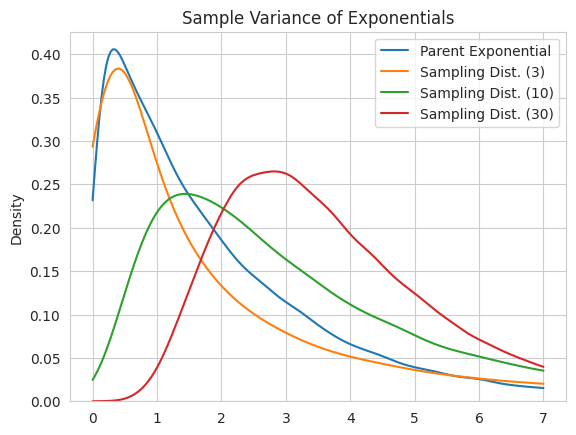
\includegraphics[width=\textwidth]{img/sample_variance_exp.png}
        \caption{}
        \label{fig:sample_variance_exp}
      \end{subfigure}
      \caption{}
      \label{fig:sample_variance_examples}
    \end{figure}
  \end{example}

\subsection{Sampling from Gaussians}

  Now if we assume that the parent distribution is Gaussian, then we can conclude some extra things and more kinds of distributions arise. Let $x_1, \ldots, x_n \sim \mathcal{N}(\mu, \sigma^2)$, with $\overline{x}_n$ the sample mean and $S^2_n$ the sample variance. Say that we want to find the distribution of $\overline{x}_n$. 
  \begin{enumerate}
    \item In the unrealistic case where we know the true $\sigma^2$, we don't even need to consider the sample variance. From the basic property of Gaussians, we know that $\overline{x}_n \sim \mathcal{N}(\mu, \sigma^2/n)$, or after standardizing, 
    \begin{equation}
      \frac{\overline{x}_n - \mu}{\sigma/\sqrt{n}} \sim \mathcal{N}(0, 1)
    \end{equation}
    \item In the realistic case where we don't know the true $\sigma^2$, we should replace it with our sample variance $S^2$, and it turns out that because of this extra uncertainty in the variance, our sampling distribution follows the student-t distribution, which can be interpreted as a mixture of Gaussians with differing variances. 
    \begin{equation}
      \frac{\overline{x}_n - \mu}{S/\sqrt{n}} \sim \mathrm{StudentT}(n-1)
    \end{equation}
  \end{enumerate}
  Now if we are interested in finding the distribution of $S^2_n$: 
  \begin{enumerate}
    \item In the unrealistic case where the know the true $\mu$, we don't need to consider the sampling distribution of $\overline{x}_n$. We have 
    \begin{equation}
      S^2_n = \frac{1}{n} \sum_{i=1}^n (x_i - \mu)^2 \sim \mathrm{Gamma}\Big( \frac{n}{2}, \frac{n}{2 \sigma^2} \Big)
    \end{equation}
    \item In the realistic case where we don't know $\mu$, we have 
    \begin{equation}
      \frac{n-1}{\sigma^2} S^2_n = \frac{1}{\sigma^2} \sum_{i=1}^n (x_i - \overline{x}_n )^2 \sim \chi^2 (n-1)
    \end{equation}
  \end{enumerate}

\subsection{Bias Variance Noise Decomposition} 

  Let's do some further analysis on this. When you take a supremum over a function class, it decomposes into 3 terms. 
  \begin{enumerate}
    \item One of which quantifies how big the function class is (more variance). 
    \item One of which quantifies the distance between the truth and the function class (bias).  
    \item One is the noise term, which is the irreducible error. 
  \end{enumerate}

  \begin{example}[Bias and Variance Tradeoff in Polynomial Regression]
    Let's motivate this by trying to fit a polynomial on some data. 
    \begin{figure}[H]
      \centering 
      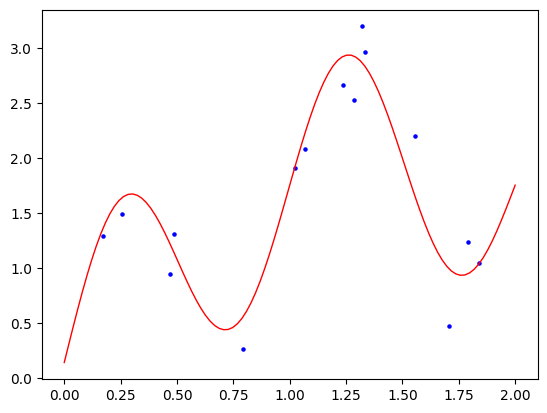
\includegraphics[scale=0.4]{img/True_data.png}
      \caption{A sample of $|\mathcal{D}| = 15$ data points are generated from the function $f(x) = \sin(2\pi x) + 2\cos (x - 1.5)$ with Gaussian noise $N(0, 0.3)$ on the interval $[0, 1]$. } 
      \label{fig:true_data}
    \end{figure}

    If we try to fit a polynomial function, how do we know which degree is best? Well the most simple thing is to just try all of them. To demonstrate this even further, I generated 10 different datasets  $\mathcal{D}$ of size $15$ taken from the same true distribution. The best fitted polynomials for each dataset is shown below. 

    \begin{figure}[H]
      \centering 
      \begin{subfigure}[b]{0.32\textwidth}
      \centering
        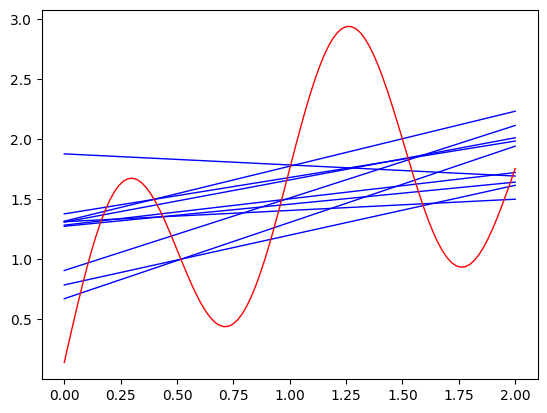
\includegraphics[width=\textwidth]{img/poly_1_fit.png}
        \caption{1st Degree}
        \label{fig:1d}
      \end{subfigure}
      \hfill 
      \begin{subfigure}[b]{0.32\textwidth}
      \centering
        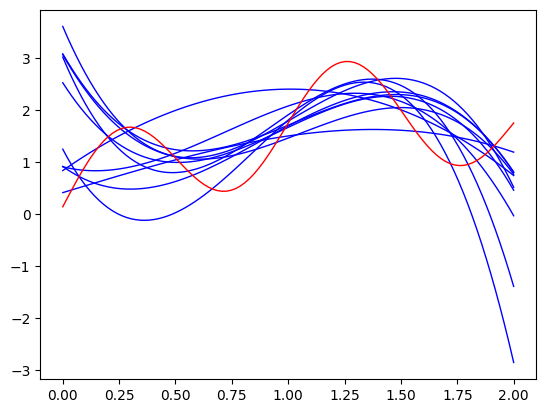
\includegraphics[width=\textwidth]{img/poly_3_fit.png}
        \caption{3rd Degree}
        \label{fig:3d}
      \end{subfigure}
      \hfill 
      \begin{subfigure}[b]{0.32\textwidth}
      \centering
        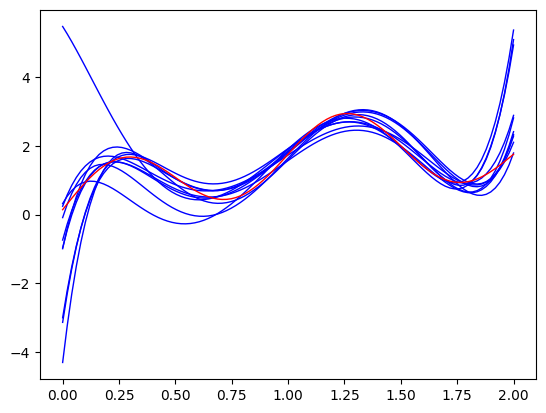
\includegraphics[width=\textwidth]{img/poly_5_fit.png}
        \caption{5th Degree}
        \label{fig:5e}
      \end{subfigure}

      \begin{subfigure}[b]{0.32\textwidth}
      \centering
        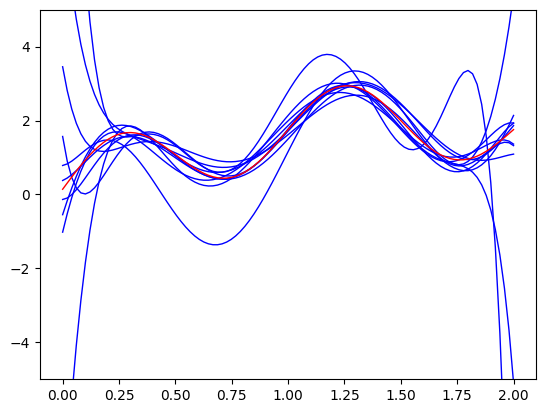
\includegraphics[width=\textwidth]{img/poly_7_fit.png}
        \caption{7th Degree}
        \label{fig:7d}
      \end{subfigure}
      \hfill 
      \begin{subfigure}[b]{0.32\textwidth}
      \centering
        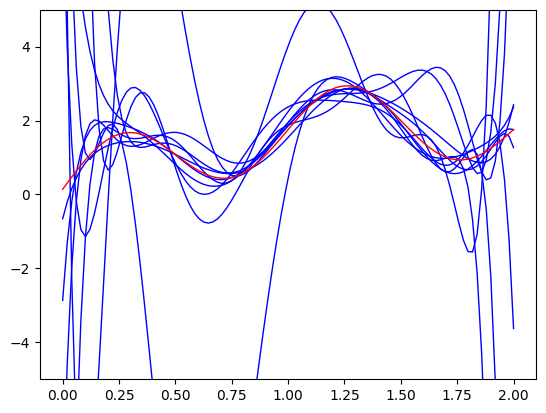
\includegraphics[width=\textwidth]{img/poly_9_fit.png}
        \caption{9th Degree}
        \label{fig:9d}
      \end{subfigure}
      \hfill 
      \begin{subfigure}[b]{0.32\textwidth}
      \centering
        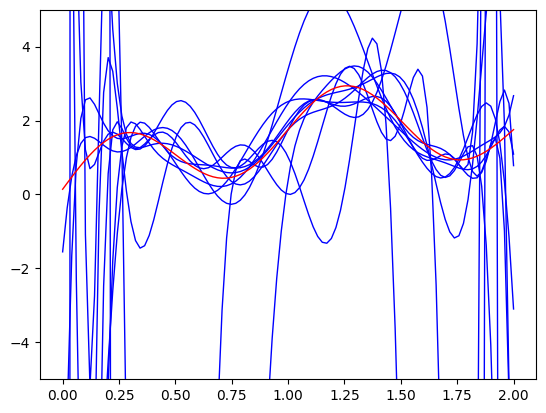
\includegraphics[width=\textwidth]{img/poly_11_fit.png}
        \caption{11th Degree}
        \label{fig:11e}
      \end{subfigure}

      \caption{Different model complexities (i.e. different polynomial degrees) lead to different fits of the data generated from the true distribution. The lower degree best fit polynomials don't have much variability in their best fits but have high bias, while the higher degree best fit polynomials have very high variability in their best fits but have low bias. The code used to generate this data is \href{code/polynomial_fitting.ipynb}{here}. }
      \label{fig:polynomial_fitting}
    \end{figure}

    We already know that the 5th degree approximation is most optimal, and the lower degree ones are \textbf{underfitting} the data, while the higher degree ones are \textbf{overfitting}. As mentioned before, we can describe the underfitting and overfitting phenomena through the bias variance decomposition. 

    \begin{enumerate}
      \item If we underfit the data, this means that our model is not robust and does not capture the patterns inherent in the data. It has a high bias since the set of function it encapsulates is not large enough to model $\mathbb{E}[Y\mid X]$. However, it has a low variance since if we were to take different samples of the dataset $\mathcal{D}$, the optimal parameters would not fluctuate. 

      \item What overfitting essentially means is that our model is too complex to the point where it starts to fit to the \textit{noise} of the data. This means that the variance is high, since different samples of the dataset $\mathcal{D}$ would cause huge fluctuations in the optimal trained parameters $\boldsymbol{\theta}$. However, the function set would be large, and thus it would be close to $\mathbb{E}[Y \mid X]$, leading to a low bias. 
    \end{enumerate}
  \end{example}
  
  \begin{example}[Polynomial Regression Continued]
    Another way to reduce the overfitting problem is if we have more training data to work with. That is, if we were to fit a 9th degree polynomial on a training set of not $N = 15$, but $N = 100$ data points, then we can see that this gives a much better fit. This makes sense because now the random variable $\mathcal{D}$, as a function of more random variables, has lower variance. Therefore, the lower variance in the dataset translates to lower variance in the optimal parameter. 

    \begin{figure}[H]
      \centering
      \begin{subfigure}[b]{0.48\textwidth}
      \centering
        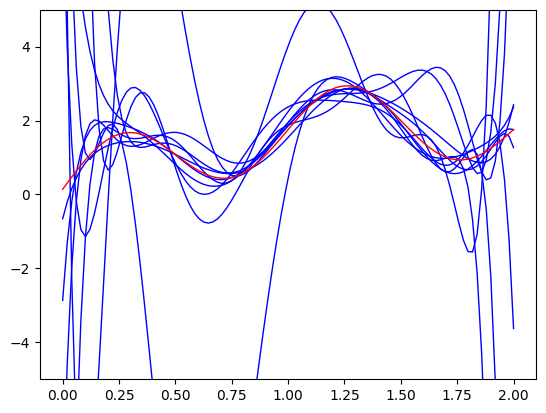
\includegraphics[width=\textwidth]{img/poly_9_fit.png}
        \caption{$M = 9, N = 15$}
        \label{fig:less_points}
      \end{subfigure}
      \hfill 
      \begin{subfigure}[b]{0.48\textwidth}
      \centering
        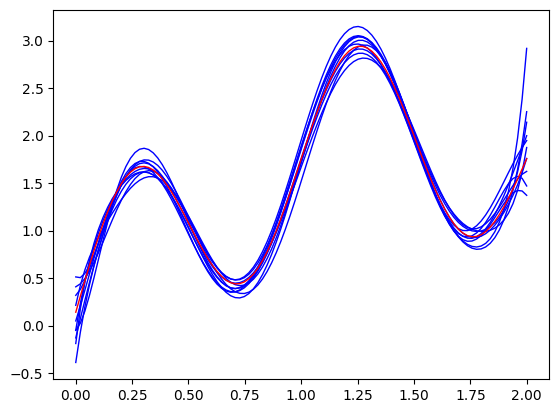
\includegraphics[width=\textwidth]{img/increased_data.png}
        \caption{$M = 9, N = 100$}
        \label{fig:more_points}
      \end{subfigure}
      \caption{Increasing the number of data points helps the overfitting problem. Now, we can afford to fit a 9th degree polynomial with reasonable accuracy.}
      \label{fig:reducing_overfitting_with_more_samples}
    \end{figure}
  \end{example}


\section{Hypothesis Testing}

  This was done for the first time as early as 1710, when a researcher tried to measure sex ratios in a population \cite{1710arbuthnot}. 
  
  A significance test is a method used to decide whether the data at hand sufficiently supports a particular hypothesis. The hypothesis to be tested is called the \textbf{alternative hypothesis}, denoted $H_1$ or $H_a$, and the status quo is called the \textbf{null hypothesis}, denoted $H_0$. Assuming that $H_0$ is true, we compute the likelihood of the data happening. If the sample is not too unlikely (past some significance level), we fail to reject $H_0$, and if there is strong evidence, we reject $H_0$. $H_0$ and $H_a$ can be devised in countless ways. 

  \begin{example}
    There are countless test statistics we can build, but here are some common examples, 
    \begin{enumerate}
      \item Proportion: Company A produces circuit boards, but 10\% of them are defective. Company B claims that they produce fewer defective circuit boards. 
      \begin{equation}
        H_0 : \, p = 0.10 \text{ versus } H_a : \, p < 0.10
      \end{equation}
      
      \item Means: It is known that the average height of boys in KIS is 176cm. Ben claims that the average height is lower than this. 
      \begin{equation}
        H_0 : \, \mu = 176 \text{ versus } H_a : \, \mu < 176
      \end{equation}
      
      \item Difference of Means: If $\mu_1$ and $\mu_2$ denote the true average breaking strengths of the same type of twine produced by two different companies. Jenny claims that the $\mu_1 - \mu_2 > 5$. 
      \begin{equation}
        H_0 : \, \mu_1 - \mu_2 = 0 \text{ versus } H_a : \, \mu_1 - \mu_2 > 5
      \end{equation}
    \end{enumerate}
  \end{example}

\subsection{One Sample Z and T Tests}

  Let us have some population $X \sim P$ and a null hypothesis that claims $H_0 : \, \mu = \theta_0$. Since we are interested in the mean, we would like to use CLT or some other theorem to determine what the distribution of the mean of $n$ samples $\overline{x}_n$ looks like (either Normal or Student T centered around $\theta_0$ and scaled down by factor of $\sqrt{n}$). When we actually sample, the value $\overline{x}_n = \hat{\theta}$ is realized, and we would like to see if sampling $\hat{\theta}$ from the distribution centered around $\theta_0$ is likely, usually after normalizing. If it isn't, then we reject $H_0$. 

  How do we decide whether to use the z-test or the t-test? It is known that $\mathrm{StudentT}(n-1)$ converges to $\mathcal{N}(0, 1)$ in distribution as $n \rightarrow +\infty$. Therefore, depending on the context of the problem, at a certain point $N$ (usually $N = 30$ or perhaps higher for skewed distributions), the difference between these two are negligible. 
  \begin{enumerate}
    \item Z-test: if we know the population variance $\sigma^2$, but it is rarely the case that we actually know $\sigma^2$. 
    \item T-test: if we do not know the population variance $\sigma^2$, which we then substitute for the sample variance $S^2$. 
    \item Z-test: if we do not know the population variance (which we substitute for $S^2$), but our sample size is greater than $N$, then we can approximate the $t$-distribution with our normal, allowing us to use the Z-test again. 
  \end{enumerate}

  In general, the alternative to the null hypothesis $H_0 : \, \theta = \theta_0$ will looks like one of the following three assertions: 
  \begin{enumerate}
    \item Two-Sided Test: $H_a : \, \theta \neq \theta_0$ 
    \item One-Sided Test: $H_a : \, \theta > \theta_0$ (in which case the null hypothesis is $\theta \leq \theta_0$) 
    \item One-Sided Test: $H_a : \, \theta < \theta_0$ (in which case the null hypothesis is $\theta \geq \theta_0$) 
  \end{enumerate}

  Now we must still quantify \textit{how} unlikely our sample mean $\theta$ must be compared to $\theta_0$ in order to reject the null hypothesis. This is where we specify our \textbf{significance level}, denoted by $\alpha$ (common values $0.10, 0.05, 0.01$). This specifies the tail-regions in which $\theta$ will land in with probability $\alpha$. Usually, working with general normal/t distributions is tedious, so we can rescale them and use their z/t-scores. 

  \begin{definition}[Z-score]
    Given a value $x$ sampled from distribution $X \sim \mathcal{N}(\mu, \sigma^2)$, its \textbf{z-score} is defined to be the number of standard deviations away from the mean. 
    \begin{equation}
      z \coloneqq \frac{x - \mu}{\sigma}
    \end{equation}
    Now given a significance level $\alpha \in [0, 1]$, let $z_\alpha$ be the value such that the measure of a standard normal distribution past $z_\alpha$ is $1 - \alpha$ (i.e. the $100\alpha$ percentile). $z_\alpha$ is called the \textbf{critical z-value}.
  \end{definition}

  \begin{definition}[T-score]
    Given a value $x$ sampled from distribution $X \sim \mathrm{StudentT}(n)$, its \textbf{t-score} is defined to be the number of standard deviations away from the mean. 
  \end{definition}

  \begin{example}
    A factory has a machine that dispenses 80mL of fluid in a bottle. An employee believes the average amount of fluid is not 80mL. Using 40 samples, he measures the average amount dispensed by the machine to be 78mL with a sample standard deviation of 2.5. 
    \begin{enumerate}
      \item Let the true mean be $\mu$ and true standard deviation be $\sigma$. The null hypothesis is $H_0 : \, \mu = 80$ and the alternative is $H_1 : \, \mu \neq 80$, making this a two-sided test. 
      
      \item We don't know the true standard deviation $\sigma$, so we must use the sample standard deviation $S$. This requires us to use the $t$-test, but since $n > 30$, we can invoke CLT and state that $\overline{x}_{40}$ is (approximately) Gaussian with mean $\mu$ and standard deviation $S / \sqrt{n}$. So, we use the $z$-test. 
      
      \item At a 95\% confidence level, we have $\alpha = 0.05$, and our rejection region is $(-\infty, z_{0.025}] \cup [z_{0.975}, +\infty)$. Since we are looking at a standard Gaussian, we have by symmetry $z_{0.025} = -1.96$ and $z_{0.975} = 1.96$, and our critical z-value is $z^\ast = 1.96$. 
      
      \item So the z-score for $78$ is 
      \begin{equation}
        z = \frac{\overline{x} - \mu_0}{s / \sqrt{n}} = \frac{78 - 80}{2.5 / \sqrt{40}} = -5.06
      \end{equation}
      which is definitely in the reject region. So this tells us that we can reject the null hypothesis with a 95\% level of confidence. 
    \end{enumerate}
  \end{example}

  \begin{example}
    A company manufactures car batteries with an average life span of 2 or more years. An engineer believes this value to be less. Using 10 samples, he measures the average life span to be 1.8 years with a standard deviation of 0.15. 
    \begin{enumerate}
      \item Let the true mean be $\mu$ and true standard deviation be $\sigma$. The null hypothesis is $H_0: \, \mu \geq 2$ and the alternative is $H_1 : \, \mu < 2$, making this a one-sided test. 
      
      \item We don't know the true standard deviation $\sigma$, so we must use the sample standard deviation $S$. This requires us to use the $t$-test, especially since $n = 10$ is not large enough for us to invoke CLT. 
      
      \item At a 99\% confidence level, we have $\alpha = 0.01$, and our rejection region is $(-\infty, t_{0.01}] = (-\infty, -2.82]$. 
      
      \item The t-score for the observed mean value is 
      \begin{equation}
        t = \frac{\overline{x} - \mu_0}{s / \sqrt{n}} = \frac{1.8 - 2}{0.15 / \sqrt{10}} = -4.22
      \end{equation}
      which is definitely in the reject region. So this tells us that we can reject the null hypothesis with a 99\% level of confidence. 
    \end{enumerate}
  \end{example}

  We may have to account for errors. There is always a chance that our evidence leads us to an incorrect conclusion, and we have names for this. 

  \begin{definition}[Errors]
    Given a hypothesis test where we look for evidence supporting our alternative claim, 
    \begin{enumerate}
      \item A \textbf{type 1 error} is when the null hypothesis is rejected, but it is true (false positive). 
      \item A \textbf{type 2 error} is when we fail to reject the null hypothesis, when it is false (false negative). 
    \end{enumerate}
  \end{definition}

\subsection{Power of a test}

\subsection{Common tests (t-test, z-test, chi-square test, F-test)}

\subsection{Multiple testing problem}


\section{Method of Moments}


\section{Maximum Likelihood Estimation}

Score function, Fisher information. 
 
\section{Bias Variance Decomposition}  

  The likelihood defines a proper loss function. Now let's try to parse the loss a bit more. It turns out that for a lot of popular loss functions, they generally decomposes into 
  \begin{equation}
    \text{Loss} = \text{Bias} + \text{Variance} + \text{Noise}
  \end{equation} 

  This decomposition is by no means exact, but it \textit{generally} holds true. This is formalized by deriving an exact decomposition of the MSE loss. This is possible because the MSE loss allows us to get an $L^2$ space, which allows for orthogonal decompositions. Unfortunately, when you have other losses, this becomes much messier because the inner product structure is not there. 

  In a more general case, when you take a supremum of risk over a function class, it decomposes into 3 terms. 
  \begin{enumerate}
    \item One of which quantifies how big the function class is (more variance). 
    \item One of which quantifies the distance between the truth and the function class (bias).  
    \item One is the noise term, which is the irreducible error. 
  \end{enumerate}

  \begin{example}[Bias and Variance Tradeoff in Polynomial Regression]
    Let's motivate this by trying to fit a polynomial on some data. 
    \begin{figure}[H]
      \centering 
      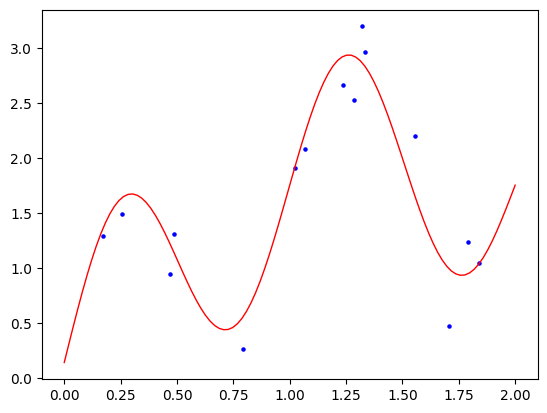
\includegraphics[scale=0.4]{img/True_data.png}
      \caption{A sample of $|\mathcal{D}| = 15$ data points are generated from the function $f(x) = \sin(2\pi x) + 2\cos (x - 1.5)$ with Gaussian noise $N(0, 0.3)$ on the interval $[0, 1]$. } 
      \label{fig:true_data}
    \end{figure}

    If we try to fit a polynomial function, how do we know which degree is best? Well the most simple thing is to just try all of them. To demonstrate this even further, I generated 10 different datasets  $\mathcal{D}$ of size $15$ taken from the same true distribution. The best fitted polynomials for each dataset is shown below. 

    \begin{figure}[H]
      \centering 
      \begin{subfigure}[b]{0.32\textwidth}
      \centering
        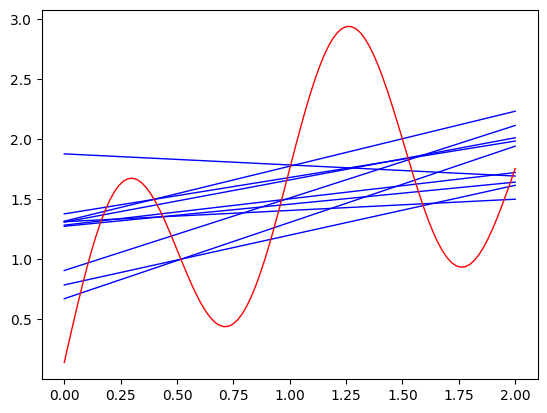
\includegraphics[width=\textwidth]{img/poly_1_fit.png}
        \caption{1st Degree}
        \label{fig:1d}
      \end{subfigure}
      \hfill 
      \begin{subfigure}[b]{0.32\textwidth}
      \centering
        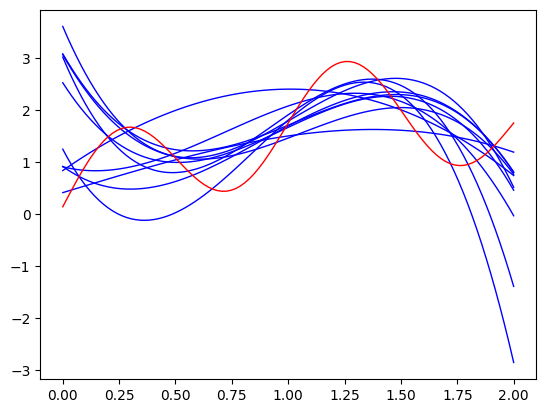
\includegraphics[width=\textwidth]{img/poly_3_fit.png}
        \caption{3rd Degree}
        \label{fig:3d}
      \end{subfigure}
      \hfill 
      \begin{subfigure}[b]{0.32\textwidth}
      \centering
        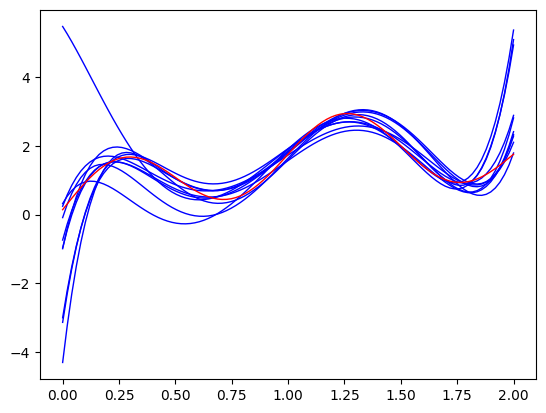
\includegraphics[width=\textwidth]{img/poly_5_fit.png}
        \caption{5th Degree}
        \label{fig:5e}
      \end{subfigure}

      \begin{subfigure}[b]{0.32\textwidth}
      \centering
        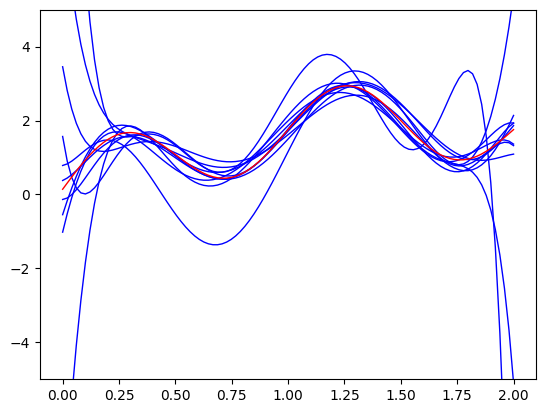
\includegraphics[width=\textwidth]{img/poly_7_fit.png}
        \caption{7th Degree}
        \label{fig:7d}
      \end{subfigure}
      \hfill 
      \begin{subfigure}[b]{0.32\textwidth}
      \centering
        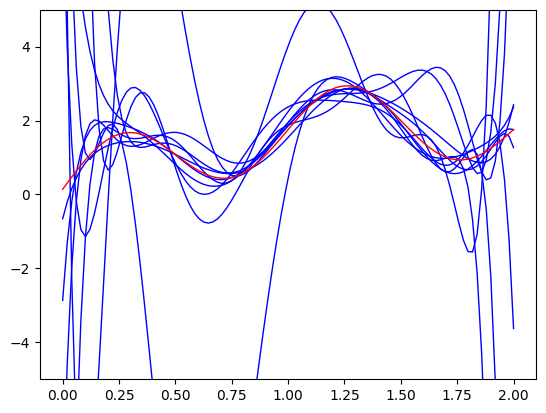
\includegraphics[width=\textwidth]{img/poly_9_fit.png}
        \caption{9th Degree}
        \label{fig:9d}
      \end{subfigure}
      \hfill 
      \begin{subfigure}[b]{0.32\textwidth}
      \centering
        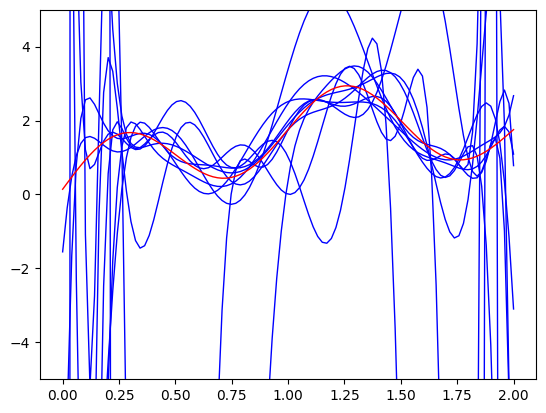
\includegraphics[width=\textwidth]{img/poly_11_fit.png}
        \caption{11th Degree}
        \label{fig:11e}
      \end{subfigure}

      \caption{Different model complexities (i.e. different polynomial degrees) lead to different fits of the data generated from the true distribution. The lower degree best fit polynomials don't have much variability in their best fits but have high bias, while the higher degree best fit polynomials have very high variability in their best fits but have low bias. The code used to generate this data is \href{code/polynomial_fitting.ipynb}{here}. }
      \label{fig:polynomial_fitting}
    \end{figure}

    We already know that the 5th degree approximation is most optimal, and the lower degree ones are \textbf{underfitting} the data, while the higher degree ones are \textbf{overfitting}. As mentioned before, we can describe the underfitting and overfitting phenomena through the bias variance decomposition. 

    \begin{enumerate}
      \item If we underfit the data, this means that our model is not robust and does not capture the patterns inherent in the data. It has a high bias since the set of function it encapsulates is not large enough to model $\mathbb{E}[Y\mid X]$. However, it has a low variance since if we were to take different samples of the dataset $\mathcal{D}$, the optimal parameters would not fluctuate. 

      \item What overfitting essentially means is that our model is too complex to the point where it starts to fit to the \textit{noise} of the data. This means that the variance is high, since different samples of the dataset $\mathcal{D}$ would cause huge fluctuations in the optimal trained parameters $\boldsymbol{\theta}$. However, the function set would be large, and thus it would be close to $\mathbb{E}[Y \mid X]$, leading to a low bias. 
    \end{enumerate}
  \end{example}
  
  \begin{example}[Polynomial Regression Continued]
    Another way to reduce the overfitting problem is if we have more training data to work with. That is, if we were to fit a 9th degree polynomial on a training set of not $N = 15$, but $N = 100$ data points, then we can see that this gives a much better fit. This makes sense because now the random variable $\mathcal{D}$, as a function of more random variables, has lower variance. Therefore, the lower variance in the dataset translates to lower variance in the optimal parameter. 

    \begin{figure}[H]
      \centering
      \begin{subfigure}[b]{0.48\textwidth}
      \centering
        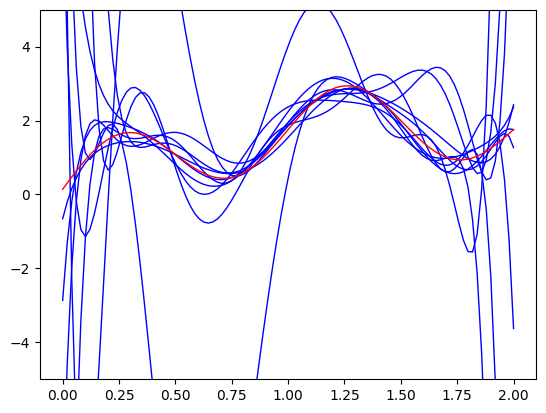
\includegraphics[width=\textwidth]{img/poly_9_fit.png}
        \caption{$M = 9, N = 15$}
        \label{fig:less_points}
      \end{subfigure}
      \hfill 
      \begin{subfigure}[b]{0.48\textwidth}
      \centering
        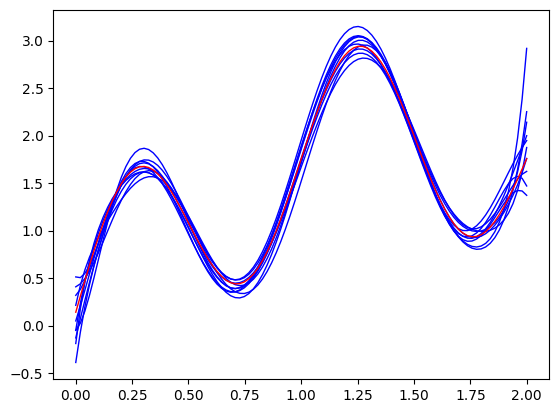
\includegraphics[width=\textwidth]{img/increased_data.png}
        \caption{$M = 9, N = 100$}
        \label{fig:more_points}
      \end{subfigure}
      \caption{Increasing the number of data points helps the overfitting problem. Now, we can afford to fit a 9th degree polynomial with reasonable accuracy.}
      \label{fig:reducing_overfitting_with_more_samples}
    \end{figure}
  \end{example}



\subsection{MSE Loss} 

  \begin{definition}[Mean Squared Error Loss]
    \label{mse_loss}
    The \textbf{MSE loss} is defined 
    \begin{equation}
      L(y, x) = (y - f(x))^2
    \end{equation}
  \end{definition}

  It is a well known fact that the true regressor---which may not be linear at all---that minimizes this loss is 
  \begin{equation}
    f^\ast (x) = \mathbb{E}[Y \mid X = x]
  \end{equation}
  which is the conditional expectation of $Y$ given $X$. This is the true regressor function, which is the best approximation of $Y$ over the $\sigma$-algebra generated by $X$. Therefore, if we consider a function class of linear predictors, we can decompose our risk, which is the distance between our estimated linear regressor and $Y$, as the sum of the distance between our estimator and the best regressor plus the distance between the best regressor and $Y$. 

  \begin{theorem}[Pythagorean's Theorem]
    The expected square loss over the joint measure $\mathbb{P}_{x, y}$ can be decomposed as 
    \begin{equation}
      \mathbb{E}_{x, y} [( y - f(x))^2] = \mathbb{E}_{x, y} [\big(y - \mathbb{E}[y \mid x]\big)^2] + \mathbb{E}_x [\big(\mathbb{E}[y \mid x] - h(x) \big)^2]
    \end{equation}
    That is, the squared loss decomposes into the squared loss of $\mathbb{E}[y \mid x]$ and $g(x)$, which is the intrinsic misspecification of the model, plus the squared difference of $y$ with its best approximation $\mathbb{E}[y \mid x]$, which is the intrinsic noise inherent in $y$ beyond the $\sigma$-algebra of $x$. 
  \end{theorem}
  \begin{proof}
    We can write 
    \begin{align}
      \mathbb{E}_{x, y} \big[ \big(y - f(x)\big)^2 \big] & = \mathbb{E}_{x, y}\big[ \big((y - \mathbb{E}[y \mid x]) + (\mathbb{E}[y \mid x] - f(x)) \big)^2 \big] \\
      & = \mathbb{E}_{x, y} [\big(y - \mathbb{E}[y \mid x]\big)^2] + \mathbb{E}_{x, y} [\{y - \mathbb{E} [y \mid x]\} \, \{ \mathbb{E}[y \mid x] - f(x) \}] \\
      & \;\;\;\;\;\;\;\;\;\;\;\;\;\;\; + \mathbb{E}_x [\big(\mathbb{E}[y \mid x] - f(x) \big)^2] \\
      & = \mathbb{E}_{x, y} [\big(y - \mathbb{E}[y \mid x]\big)^2] + \mathbb{E}_x [\big(\mathbb{E}[y \mid x] - f(x) \big)^2]
    \end{align}
    where the middle term cancels out due to the tower property. 
  \end{proof}

  Note that since $\mathbb{E}[\big(\mathbb{E}[Y \mid X] - g(X) \big)^2]$ is the misspecification of the model, we cannot change this (positive) constant, so $\mathbb{E}\big[ \big(Y - g(X)\big)^2 \big] \geq \mathbb{E}[(Y - \mathbb{E}[Y \mid X])^2]$, with equality achieved when we perfectly fit $g$ as $\mathbb{E}[Y \mid X]$ (i.e. the model is well-specified). Therefore, denoting $\mathcal{F}$ as the set of all $\sigma(X)$-measurable functions, then the minimum of the loss is attained when 
  \begin{equation}
    \argmin_{g \in \mathcal{F}} \mathbb{E}[L] = \argmin_{g \in \mathcal{F}} \mathbb{E} \big[ \big(Y - g(X)\big)^2 \big] = \mathbb{E}[Y \mid X]
  \end{equation}
  Essentially, we have decomposed our risk to a part that we can optimize and a part that we cannot, i.e. the intrinsic noise. 

  \begin{corollary}[Sufficient to Estimate Conditional Expectation]
    Minimizing the prediction risk is equivalent to minimizing the risk of our estimator to the conditional distribution. 
    \begin{equation}
      \argmin_{f \in \mathcal{F}} R(f) = \argmin_{f \in \mathcal{F}} \mathbb{E}_{x, y} \left[ (\mathbb{E}[y|x] - f(x))^2 \right]
    \end{equation}
  \end{corollary}
  
  Even though this example is specific for the mean squared loss, this same decomposition, along with the bias variance decomposition, exists for other losses. It just happens so that the derivations are simple for the MSE, which is why this is introduced first. However, the derivations for other losses are much more messy, and sometimes may not hold rigorously. However, the general intuition that more complex models tend to overfit (higher variance) still hold true. 

  Let's try to decompose this even more. In frequentist inference, we take a dataset $\mathcal{D}$ and optimize $\hat{f}$ that minimizes this empirical risk. Therefore, for a given $\mathcal{D}$, $\hat{f} = \hat{f}(\mathcal{D})$ is determined, and if $\mathcal{D} = (x^{(i)}, y^{(i)})^n$ is a random variable, then $\hat{f}$ is also a random variable, which we will denote as $\hat{f}_{\mathcal{D}}$ for clarity. It is useful to think of $\mathcal{D}$ as a random variable because by seeing how $\hat{f}_{\mathcal{D}}$ varies as the dataset changes, we can measure the uncertainty in our estimate of $\hat{f}_{\mathcal{D}}$ through $\mathcal{D}$.\footnote{If this didn't make sense to you, consider the following thought experiment. Suppose we had a large number of datasets each of size $N$ and each drawn independently from the joint distribution $X \times Y$. For any given dataset $\mathcal{D}$, we can run our learning algorithm and obtain our best fit function $\hat{f}_{\mathcal{D}}$. Different datasets from the ensemble will give different functions and consequently different values of the squared loss. }

  \begin{lemma}[Conditional Prediction Risk] 
    Our conditional prediction risk is 
    \begin{equation}
      r(\mathcal{D}) = \mathbb{E}_{x, y} \left[ (\mathbb{E}[y \mid x] - \hat{f}(x))^2 \mid \mathcal{D} \right]
    \end{equation}
    If $\mathcal{D}$ is fixed, then this is a real number. If $\mathcal{D}$ is a random variable, then this is a real-valued random variable. 
  \end{lemma} 

  Ideally, we would like two things. 
  \begin{enumerate}
    \item \textit{Low Bias}. The average prediction we get over all $\hat{f}_{\mathcal{D}}$ trained on all possible samples of dataset $\mathcal{D}$ should be similar to our best regressor. That is, 
    \begin{equation}
      \mathbb{E}_{\mathcal{D}} \left[ \mathbb{E}_{x, y} \left[ (\mathbb{E}[y \mid x] - \hat{f}_{\mathcal{D}}(x))^2 \right] \right]
    \end{equation}
    should be as low as possible. 

    \item \textit{Low Variance}. The variance of our conditional prediction risk  
    \begin{equation}
      \Var_{\mathcal{D}} \left[ \mathbb{E}_{x, y} \left[ (\mathbb{E}[y \mid x] - \hat{f}_{\mathcal{D}}(x))^2 \right] \right]
    \end{equation}
    should be as low as possible. That is, we may get very low bias for one dataset $\mathcal{D}$, but if we sampled a different dataset, we should not expect the bias to explode. 
  \end{enumerate}

  Unfortunately, having both low bias \textit{and} low variance is not possible, and we wish to show that now. 

  \begin{theorem}[Bias Variance Decomposition Under MSE Loss]
    The expected optimal MSE loss decomposes to 
    \begin{equation}
      \mathbb{E}_{\mathcal{D}} \left[ (\mathbb{E}[y \mid x] - \hat{f}_\mathcal{D} (x))^2 \right] = \underbrace{ \big( \mathbb{E}[y \mid x] - \mathbb{E}_{\mathcal{D}} [\hat{f}_\mathcal{D} (x)] \big)^2}_{(\text{bias of } \hat{f}_{\mathcal{D}})^2} + \underbrace{ \mathbb{E}_\mathcal{D} \big[ \big( \mathbb{E}_\mathcal{D} [\hat{f}_\mathcal{D} (x)] - \hat{f}_\mathcal{D} (x) \big)^2 \big]}_{\text{variance of } \hat{f}_{\mathcal{D}}}
    \end{equation}
  \end{theorem}
  \begin{proof}
    Consider the term $\big(\mathbb{E}[y \mid x] - \hat{f}_{\mathcal{D}}(x) \big)^2$ above, which models the discrepancy in our optimized hypothesis and the best approximation. We take $\mathbb{E}_{\mathcal{D}} [ \hat{f}_{\mathcal{D}} (x)]$\footnote{Over all datasets $\mathcal{D}$, there will be a function $h_{{\boldsymbol{\theta}}; \mathcal{D}}$, and averaged over all datasets $\mathcal{D}$ is $\mathbb{E}_\mathcal{D} [ \hat{f}_{\mathcal{D}}]$. } So we can split the term into 

    \begin{align}
      \big(\mathbb{E}[y \mid x] - \hat{f}_{\mathcal{D}} (x) \big)^2 & =  \big[ \big( \mathbb{E}[y \mid x] - \mathbb{E}_\mathcal{D} [\hat{f}_{\mathcal{D}} (x)] \big) + \big( \mathbb{E}_\mathcal{D} [\hat{f}_{\mathcal{D}} (x)] - \hat{f}_{\mathcal{D}} (x) \big) \big]^2 \\
      & = \big( \mathbb{E}[y \mid x] - \mathbb{E}_\mathcal{D} [\hat{f}_{\mathcal{D}} (x)] \big)^2 + \big( \mathbb{E}_\mathcal{D} [\hat{f}_{\mathcal{D}} (x)] - \hat{f}_{\mathcal{D}} (x) \big)^2 \\
      & \;\;\;\;\;\;\;\; + 2 \big( \mathbb{E}[y \mid x] - \mathbb{E}_\mathcal{D} [\hat{f}_{\mathcal{D}} (x)] \big) \big( \mathbb{E}_\mathcal{D} [\hat{f}_{\mathcal{D}} (x)] - \hat{f}_{\mathcal{D}} (x) \big) 
    \end{align}

    Now take the expectation over $\mathcal{D}$, and for the third term, note that $\big( \mathbb{E}[y \mid x] - \mathbb{E}_\mathcal{D} [\hat{f}_{\mathcal{D}} (x)] \big)$ is constant with respect to $\mathbb{D}$ anyways, so we can take it out of the expectation. Therefore, 
    \begin{align}
      \mathbb{E}_{\mathcal{D}} \big[ \big( \mathbb{E}[y \mid x] - & \mathbb{E}_\mathcal{D} [\hat{f}_{\mathcal{D}} (x)] \big) \big( \mathbb{E}_\mathcal{D} [\hat{f}_{\mathcal{D}} (x)] - \hat{f}_{\mathcal{D}} (x) \big) \big] \\
      & = \big( \mathbb{E}[y \mid x] - \mathbb{E}_\mathcal{D} [\hat{f}_{\mathcal{D}} (x)] \big) \, \mathbb{E}_{\mathcal{D}} \big[ \mathbb{E}_\mathcal{D} [\hat{f}_{\mathcal{D}} (x)] - \hat{f}_{\mathcal{D}} (x) \big] \\ 
      & = \big( \mathbb{E}[y \mid x] - \mathbb{E}_\mathcal{D} [\hat{f}_{\mathcal{D}} (x)] \big) \cdot 0 = 0
    \end{align} 
  \end{proof} 

  Let's parse these terms a bit more. 
  \begin{enumerate}
    \item The bias $\mathbb{E}[y \mid x] - \mathbb{E}_{\mathcal{D}} [\hat{f}_\mathcal{D} (x)]$ is a random variable of $x$ that measures the difference between the average of our learned predictor $\mathbb{E}_{\mathcal{D}} [\hat{f}_\mathcal{D} (x)]$ and the true regressor $\mathbb{E}[y \mid x]$. 

    \item The variance $\mathbb{E}_\mathcal{D} \big[ \big( \mathbb{E}_\mathcal{D} [\hat{f}_\mathcal{D} (x)] - \hat{f}_\mathcal{D} (x) \big)^2 \big]$ is a random variable of $x$ that measures the variability of our learned functions $\hat{f}_{\mathcal{D}}$ around our mean $\mathbb{E}_\mathcal{D} [\hat{f}_\mathcal{D} (x)]$. 
  \end{enumerate}

  Therefore, we can substitute this back into our Pythagoras decomposition, where we must now take the expected bias and the expected variance over $x$ to get a form like 
  \begin{equation}
    \text{Expected Loss} = (\text{Expected Bias})^2 + \text{Expected Variance} + \text{Noise}
  \end{equation}

  \begin{corollary}[Bias Variance Decomposition of Expected MSE Loss] 
    \label{bias_variance_mse}
    The expected optimal MSE loss decomposes to 
    \begin{align}
      \mathbb{E}_{\mathcal{D}} \mathbb{E}_{x, y} \big[ (y - \hat{f}_{\mathcal{D}}(x))^2 \big] 
      & = \mathbb{E}_{x} \big[ \underbrace{ \big( \mathbb{E}[y \mid x] - \mathbb{E}_{\mathcal{D}} [\hat{f}_\mathcal{D} (x)] \big)^2}_{\text{(expected bias)}^2} \big] + \underbrace{ \mathbb{E}_\mathcal{D} \big[ \mathbb{E}_{x} \big[ \big( \mathbb{E}_\mathcal{D} [\hat{f}_\mathcal{D} (x)] - \hat{f}_\mathcal{D} (x) \big)^2 \big] \big]}_{\text{expected variance}} \\ 
      & \;\;\;\;\;\;\;\;\;\;\;\;\;\;\;\;\;\;\;\;\;\;\;\;\; + \underbrace{\mathbb{E}_{x, y} [(y - \mathbb{E}[y \mid x])^2]}_{\text{noise}}
    \end{align}
  \end{corollary}
  \begin{proof}
    By taking the expectation over $x$ and swapping the expectations (since $x$ and $\mathcal{D}$ are independent), and finally substituting back to Pythagoras decomposition, we get the following. 
  \end{proof}
  
\subsection{MAE Loss} 

  

 
\section{Confidence Intervals}

  Recall that the central limit theorem says that given a sequence of iid random variables $x_1, \ldots, x_n$ coming from a random variable with true mean $\mu$ and variance $\sigma^2$, the sample mean is similar to a $\mathcal{N}(\mu, \sigma^2 / n)$ random variable. That is, the sample mean converges in distribution 
  \begin{equation}
    \overline{X}_n \xrightarrow{dist} \mathcal{N} \Big( \mu, \frac{\sigma^2}{n} \Big)
  \end{equation}
  as $n \rightarrow \infty$. Another way to state it is that the normalized sample mean is similar to a standard Gaussian. 
  \begin{equation}
    \frac{\overline{x}_n - \mu}{\sigma_{\overline{x}_n}} = \frac{\overline{x}_n - \mu}{\sigma / \sqrt{n}} \xrightarrow{dist} \mathcal{N}(0, 1)
  \end{equation}
  So, given that we have enough samples, I will perfectly understand its fluctuations. Now let's introduce some definitions that will allow us to unify some ideas into simpler notation: the realized value $x$, the number of standard deviations it is away from the mean, and the probability that it takes that value (or more extreme). 

  \begin{definition}[z-score]
    Given a $\mathcal{N}(\mu, \sigma^2)$ distribution, the \textbf{z-score} of a number $x \in \mathbb{R}$ is defined to be the number of standard deviations away from the mean. 
    \begin{equation}
      z = \frac{x - \mu}{\sigma}
    \end{equation}
  \end{definition}

  \begin{definition}[Percentile]
    Given $X \sim \mathcal{N}(0, 1)$ and significance level $\alpha \in [0, 1]$, let us define $q_{\alpha} \in \mathbb{R}$ as the point where 
    \begin{equation}
      \mathbb{P}(X \geq q_{\alpha}) = \alpha
    \end{equation}
    i.e. the $100\alpha$th percentile of the standard normal. Note that given $X \sim \mathcal{N}(0, 1)$, we have 
    \begin{equation}
      \mathbb{P} (|X| > q_{\alpha/2}) = \alpha
    \end{equation}
  \end{definition}

  Now given $x_1, \ldots, x_n$ from a population $X$ with mean $\mu$ and standard deviation $\sigma$, let $\overline{x}_n$ be the sampling distribution of the mean. By virtue of the central limit theorem, we can write
  \begin{equation}
    \mathbb{P} \bigg( \bigg| \frac{\overline{X}_n - \mu}{\sigma / \sqrt{n}} \bigg| \geq q_{\alpha/2} \bigg) \approx \alpha \iff \mathbb{P} \bigg( \bigg| \frac{\overline{X}_n - \mu}{\sigma \sqrt{n}} \bigg| \leq q_{\alpha/2} \bigg) \approx 1 - \alpha
  \end{equation}
  which implies that with probability $1 - \alpha$, we have 
  \begin{equation}
    \overline{X}_n \in \bigg[ \mu - q_{\alpha/2} \frac{\sigma}{\sqrt{n}}, \mu + q_{\alpha/2} 
    \frac{\sigma}{\sqrt{n}} \bigg] \iff \mu \in \bigg[ \overline{X}_n - q_{\alpha/2} \frac{\sigma}{\sqrt{n}}, \overline{X}_n + q_{\alpha/2} \frac{\sigma}{\sqrt{n}} \bigg]
  \end{equation}
  This is how we construct a confidence interval. In other words, as $n$ becomes large (ideally at least $30$), the probability that an interval around our sample mean contains the actual mean $\mu$ can be approximated by a Gaussian. But note that CI requires to know the actual standard deviation $\sigma$. There are three ways to deal with this: 
  \begin{enumerate}
    \item This may actually be known from the start, especially if we are working with calibrated devices with standard devices that have been experimentally verified.

    \item We can simply bound $\sigma$, depending on what kind of random variable we are working with. For example, given $X \sim \mathrm{Bernoulli}(p)$, its standard deviation is bounded by $\sigma = \sqrt{p (1 - p)} \leq \frac{1}{2}$, so we can create a confidence interval that is larger than any other confidence interval we can make if we had known the true $\sigma$. 
    \begin{equation}
      p \in \bigg[ \overline{X}_n - q_{\alpha/2} \, \frac{1}{2 \sqrt{n}}, \overline{X}_n + q_{\alpha/2} \,\frac{1}{2 \sqrt{n}} \bigg]
    \end{equation}

    \item We can approximate $\sigma$ with the sample standard deviation $S$, which turns out to be an unbiased estimator. 
  \end{enumerate}

  \begin{example}[Proportion of Right-Side Kissers]
    We have observed $80$ out of $124$ right-side kisses, resulting in a sample estimate of $\widehat{p} = 0.645$. Given that we want a confidence interval of $95\%$, we want an $\alpha = 0.05$, implying a the value $q_{\alpha/2} = q_{0.025} = 1.96$. So, with probability $0.95$, we have 
    \begin{equation}
      p \in \bigg[ 0.645 - \frac{1.96}{2 \sqrt{124}}, 0.645 + \frac{1.96}{2 \sqrt{124}} \bigg] = [ 0.56, 0.73 ]
    \end{equation}
    If we had, say $3$ observations, rather than $124$, we would have a $95\%$ confidence interval of $p \in [0.10, 1.23]$, which is terrible, but in this case even CLT is not valid. 
  \end{example}

  \begin{example}[Proportion of Voters]
    Given that we sample $n = 100$ people from a city's population to ask whether they support candidate A or B, we have $54$ people who support candidate $A$, so $\widehat{p} = 0.54$. Say that we want a 95\% confidence interval, which leads to $q_{\alpha /2} = q_{0.025} = 1.96$. So, with probability $0.95$, we have 
    \begin{equation}
      p \in \bigg[ 0.54 - 1.96\,\frac{\sigma}{\sqrt{100}}, 0.54 + 1.96\,\frac{\sigma}{\sqrt{100}} \bigg]
    \end{equation}
    and by substituting $\sigma$ for $S = \sqrt{0.54 (1 - 0.54)} \approx 0.5$, we get 
    \begin{equation}
      p \in \bigg[ 0.54 - 1.96\,\frac{0.284}{\sqrt{100}}, 0.54 + 1.96\,\frac{0.284}{\sqrt{100}} \bigg] = [0.44, 0.64]
    \end{equation}
  \end{example}

  An interpretation of confidence intervals is that if you keep on sampling $\overline{x}$ or $\widehat{p}$ and construct 95\% CIs, then 95\% of the time these intervals will contain the true mean $\mu$ or proportion $p$ (or more if we had bounded the CI with a bigger interval). 

  \begin{example}
    We survey 6250 teachers to ask whether they think computers are essential for teaching. 250 were randomly selected and 142 felt that they were essential. Let's construct a 99\% confidence interval for the proportion of teachers who felt that computers were essential. We would like to construct a CI for the true $\mu = p$, and we have $\overline{x} = 142/250 = 0.568$. 
    \begin{enumerate}
      \item 99\% confidence corresponds to $\alpha = 0.01$, which corresponds to a z-score of $q_{\alpha/2} = 2.576$. 
      \item The parent distribution is $\mathrm{Bernoulli}(p)$, with $\mu = p$ and $\sigma = \sqrt{p (1 - p)}$. The sampling distribution of $\overline{x}$ has $\mu_{\overline{x}} = p$ also and $\sigma_{\overline{x}} = \sigma / \sqrt{n}$. 
      \item We need to know the details of the sampling distribution, but we don't know $\sigma$, which is needed to calculate $\sigma_{\overline{x}}$. However, we can estimate it using the sample standard deviation $S = \sqrt{0.568 (1 - 0.568)} = 0.5$. 
      \item Our sampling distribution has standard deviation $\sigma_{\overline{x}} \approx S / \sqrt{n} = 0.5 / \sqrt{250} = 0.031$, and our z-score was $2.576$, so our 99\% confidence interval is $2.576$ standard deviations from our mean. That is, with probability $0.99$, 
      \begin{equation}
        p \in \big[ 0.568 - 2.576 \cdot 0.031, 0.568 + 2.576 \cdot 0.031 \big] = \big[ 0.488144, 0.647856 \big]
      \end{equation}
    \end{enumerate}
  \end{example}

\subsection{CIs for means, proportions, and variances}

\subsection{Bootstrap confidence intervals}


\section{Cross Validation} 

  We have understood the theoretical foundations of overfitting and underfitting with the bias variance decomposition. But in practice, we don't have an ensemble of datasets; we just have one. Therefore, we don't actually know what the bias, the variance, or the noise is at all. Therefore, how do we actually \textit{know} in practice when we are underfitting or overfitting? Easy. We just split our dataset into 2 different parts: the training set and testing sets. 
  \begin{equation}
    \mathcal{D} = \mathcal{D}_{train} \sqcup \mathcal{D}_{test}
  \end{equation}
  What we usually have is a \textbf{training set} that allows us to train the model, and then to check its performance we have a \textbf{test set}. We would train the model on the training set, where we will always minimize the loss, and then we would look at the loss on the test set. Though we haven't made a testing set, since we know the true model let us just generate more data and use that as our testing set. For each model, we can calculate the optimal $\boldsymbol{\theta}$, which we will denote $\boldsymbol{\theta}^\ast$, according to the \textbf{root mean squared loss}
  \begin{equation}
    h_{\boldsymbol{\theta}^\ast} = \argmin_{h_{\boldsymbol{\theta}}} \sqrt{ \frac{1}{N} \sum_{i=1}^N \big( y^{(i)} - h_{\boldsymbol{\theta}} (\mathbf{x}^{(i)}) \big)^2 }
  \end{equation}
  where division of $N$ allows us to compare different sizes of datasets on equal footing, and the square root ensures that this is scaled correctly. Let us see how well these different order models perform on a separate set of data generated by the same function with Gaussian noise. 

  \begin{figure}[H]
    \centering
    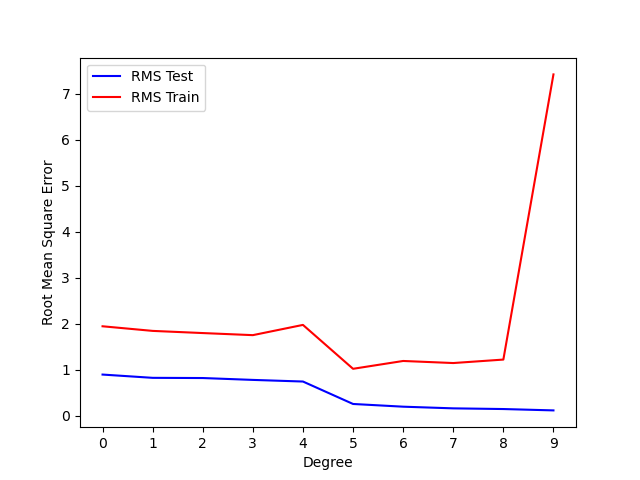
\includegraphics[scale=0.4]{img/Degree_vs_RMS.png}
    \caption{We can see that the RMS decreases monotonically on the training error as more complex functions become more fine-tuned to the data. However, when we have a $9$th degree polynomial the RMS for the testing set dramatically increases, meaning that this model does not predict the testing set well, and performance drops. }
    \label{fig:poly_deg_vs_rms}
  \end{figure}

  Now we know that a more complex model (i.e. that captures a greater set of functions) is not necessarily the best due to overfitting. Therefore, researchers perform \textbf{cross-validation} by taking the training set $(\mathcal{X}, \mathcal{Y})$. We divide it into $S$ equal pieces 
  \begin{equation}
    \bigcup_{s=1}^S D_s = (\mathcal{X}, \mathcal{Y})
  \end{equation}
  Then, we train the model $\mathcal{M}$ on $S-1$ pieces of the data and then test it across the final piece, and do this $S$ times for every test piece, averaging its perforance across all $S$ test runs. Therefore, for every model $\mathcal{M}_k$, we must train it $S$ times, for all $K$ models, requiring $KS$ training runs. If data is particularly scarce, we set $S = N$, called the \textbf{leave-one-out} technique. Then we just choose the model with the best average test performance. 

  The following result shows that cross-validation (data splitting) leads to an estimator with risk nearly as good as the best model in the class. 


  \begin{theorem}[Gyorfi, Kohler, Krzyak, Walk (2002)]
    Let $\mathcal{M} = \{m_h\}$ be a finite class of regression estimators indexed by a parameter $h$, with $m$ being the true risk minimizer, $m_{\hat{h}}$ being the empirical risk minimizer over the whole dataset $\mathcal{D}$, and $m_{H}$ being the empirical risk minimizer over the test set $\mathcal{D}_{\mathrm{test}}$ for ordinary least squares loss. 
    \begin{align}
      m_H & = \argmin_{m_h} \frac{1}{N} \sum_{i \in \mathcal{D}_{\mathrm{test}}} (y_i - m_h(x_i))^2 \\ 
      m_{\hat{h}} & = \argmin_{m_h} \frac{1}{N} \sum_{i \in \mathcal{D}} (y_i - m_h(x_i))^2 
    \end{align}
    If the data $Y_i$ and estimators are bounded by $L$, then for any $\delta > 0$, we have 
    \begin{equation}
      \mathbb{E} \int |m_H (x) - m(x)|^2 \,d\mathbb{P}(x) \leq (1 + \delta) \mathbb{E} \int |m_{\hat{h}} (x) - m(x) |^2 \,d \mathbb{P}(x) + \frac{C (1 + \log{|M|})}{n}
    \end{equation}
    where $c = L^2 (16/\delta + 35 + 19\delta)$. 
  \end{theorem}

  \begin{code}[Minimal Example of Train Test Split in scikit-learn]
    To implement this in scikit-learn, we want to use the \texttt{train\_test\_split} class. We can also set a random state parameter to reproduce results. 
    \begin{lstlisting}
      from sklearn.model_selection import train_test_split 

      # Split into training (80\%) and test (20\%) data 
      X_train, X_test, Y_train, Y_test = train_test_split(X, Y, test_size=0.2, random_state=66)
    \end{lstlisting}
  \end{code}

  However, this process requires a lot of training runs and therefore may be computationally infeasible. Therefore, various \textbf{information criterion} has been proposed to efficiently select a model. 

\subsection{Leave 1 Out Cross Validation} 

  \subsubsection{Generalized (Approximate) Cross Validation} 

  \subsubsection{Cp Statistic}

\subsection{K Fold Cross Validation}


\section{Information Criteria}



\bibliography{./bibfile}
\bibliographystyle{alpha}
\end{document}
